% Options for packages loaded elsewhere
\PassOptionsToPackage{unicode}{hyperref}
\PassOptionsToPackage{hyphens}{url}
%
\documentclass[
  9pt,
  ignorenonframetext,
]{beamer}
\usepackage{pgfpages}
\setbeamertemplate{caption}[numbered]
\setbeamertemplate{caption label separator}{: }
\setbeamercolor{caption name}{fg=normal text.fg}
\beamertemplatenavigationsymbolsempty
% Prevent slide breaks in the middle of a paragraph
\widowpenalties 1 10000
\raggedbottom
\setbeamertemplate{part page}{
  \centering
  \begin{beamercolorbox}[sep=16pt,center]{part title}
    \usebeamerfont{part title}\insertpart\par
  \end{beamercolorbox}
}
\setbeamertemplate{section page}{
  \centering
  \begin{beamercolorbox}[sep=12pt,center]{part title}
    \usebeamerfont{section title}\insertsection\par
  \end{beamercolorbox}
}
\setbeamertemplate{subsection page}{
  \centering
  \begin{beamercolorbox}[sep=8pt,center]{part title}
    \usebeamerfont{subsection title}\insertsubsection\par
  \end{beamercolorbox}
}
\AtBeginPart{
  \frame{\partpage}
}
\AtBeginSection{
  \ifbibliography
  \else
    \frame{\sectionpage}
  \fi
}
\AtBeginSubsection{
  \frame{\subsectionpage}
}
\usepackage{lmodern}
\usepackage{amsmath}
\usepackage{ifxetex,ifluatex}
\ifnum 0\ifxetex 1\fi\ifluatex 1\fi=0 % if pdftex
  \usepackage[T1]{fontenc}
  \usepackage[utf8]{inputenc}
  \usepackage{textcomp} % provide euro and other symbols
  \usepackage{amssymb}
\else % if luatex or xetex
  \usepackage{unicode-math}
  \defaultfontfeatures{Scale=MatchLowercase}
  \defaultfontfeatures[\rmfamily]{Ligatures=TeX,Scale=1}
\fi
\usetheme[]{Goettingen}
\usecolortheme{rose}
% Use upquote if available, for straight quotes in verbatim environments
\IfFileExists{upquote.sty}{\usepackage{upquote}}{}
\IfFileExists{microtype.sty}{% use microtype if available
  \usepackage[]{microtype}
  \UseMicrotypeSet[protrusion]{basicmath} % disable protrusion for tt fonts
}{}
\makeatletter
\@ifundefined{KOMAClassName}{% if non-KOMA class
  \IfFileExists{parskip.sty}{%
    \usepackage{parskip}
  }{% else
    \setlength{\parindent}{0pt}
    \setlength{\parskip}{6pt plus 2pt minus 1pt}}
}{% if KOMA class
  \KOMAoptions{parskip=half}}
\makeatother
\usepackage{xcolor}
\IfFileExists{xurl.sty}{\usepackage{xurl}}{} % add URL line breaks if available
\IfFileExists{bookmark.sty}{\usepackage{bookmark}}{\usepackage{hyperref}}
\hypersetup{
  pdftitle={BIOS6643 Longitudinal},
  pdfauthor={EJC},
  hidelinks,
  pdfcreator={LaTeX via pandoc}}
\urlstyle{same} % disable monospaced font for URLs
\newif\ifbibliography
\usepackage{longtable,booktabs}
\usepackage{calc} % for calculating minipage widths
\usepackage{caption}
% Make caption package work with longtable
\makeatletter
\def\fnum@table{\tablename~\thetable}
\makeatother
\setlength{\emergencystretch}{3em} % prevent overfull lines
\providecommand{\tightlist}{%
  \setlength{\itemsep}{0pt}\setlength{\parskip}{0pt}}
\setcounter{secnumdepth}{-\maxdimen} % remove section numbering
\AtBeginSubsection{}
\AtBeginSection{}
\ifluatex
  \usepackage{selnolig}  % disable illegal ligatures
\fi

\title{BIOS6643 Longitudinal}
\subtitle{L17 Ordinal logistic regression}
\author{EJC}
\date{}
\institute{Department of Biostatistics \& Informatics}

\begin{document}
\frame{\titlepage}

\begin{frame}[allowframebreaks]
  \tableofcontents[hideallsubsections]
\end{frame}
\hypertarget{ordinal-regression}{%
\section{Ordinal regression}\label{ordinal-regression}}

\begin{frame}{Topics for these notes:}
\protect\hypertarget{topics-for-these-notes}{}
\begin{itemize}
\tightlist
\item
  Ordinal logistic regression
\end{itemize}

Associated reading: as of now, the course notes do not have more
information than what is here.
\end{frame}

\hypertarget{case-study}{%
\section{Case study}\label{case-study}}

\begin{frame}{Case Study}
\protect\hypertarget{case-study-1}{}
``Since 2001, 3 million soldiers have deployed to Southwest Asia (SWA),
with exposure to inhalants that cause respiratory disease. Department of
Defense uses standard occupational codes, termed Military Occupational
Specialty (MOS), to classify military personnel by job/training. We
characterized Marine MOS by estimated exposure to inhalational hazards.
We developed an MOS-exposure matrix containing five major deployment
inhalational hazards--sandstorms, burn pits, exhaust fumes, combat dust,
occupational VDGF (vapor, dust, gas, fumes)--plus time worked outdoors.
A 5 member expert panel of two physician deployment veterans and three
occupational pulmonologists independently ranked 38 Marine MOS codes for
estimated exposure intensity (3=high, 2=medium, 1=low) to each hazard.''
From Pepper et al., 2017.
\end{frame}

\begin{frame}{}
\protect\hypertarget{section}{}
The MOS occupational codes (or MOS\_num) are numbered 1 through 38, for
convenience, but they relate to specific job types. For example,
1=personnel and administration, 2=intelligence, 3=infantry, etc.

Our data follows this form, for a given inhalation hazard:

\begin{longtable}[]{@{}lllllll@{}}
\toprule
Rater & MOS1 & MOS2 & MOS3 & MOS4 & MOS5 & \ldots{}\tabularnewline
\midrule
\endhead
1 & 1 & 1 & 3 & 2 & 1 &\tabularnewline
2 & 1 & 1 & 3 & 1 & 1 &\tabularnewline
3 & 1 & 2 & 3 & 2 & 1 &\tabularnewline
\ldots{} & & & & & &\tabularnewline
\bottomrule
\end{longtable}

The outcome is ordinal and given that there are only 3 levels (3 is high
exposure, 2 is medium, 1 is low), we consider a model that is
specialized for this type of outcome.
\end{frame}

\begin{frame}{}
\protect\hypertarget{section-1}{}
A GzLMM that can be used to fit our data has the form
\(\lambda_{ijk} = log\Big[\frac {P(Y_{ij} \leq k\ |\ b_i,\ b_j)} {1-P(Y{_ij} \leq k\ |\ b_i,\ b_j)}\Big] = \alpha_k + b_i + b_j\),

where \(i\) = MOS\_num, \(j\)= rater, and \(k\) is outcome level;
\(\alpha_k,\ k=1,\ ...,\ K-1\) are strictly increasing intercepts; bi
and bj are random intercepts for MOS\_num and rater, respectively.

In order to get estimates that are commensurate with increasing levels
of the outcome, we can reverse the inequalities to obtain
\(\lambda_{ijk}^c = log \Big[ \frac {P(Y_{ij} \geq\ k\ |\ b_i,\ b_j)} {1 - P(Y_{ij} \geq k\ |\ b_i,\ b_j)}\Big]=\alpha _k+b_i+b_j\).

This is the model we will fit for the application. We achieve this model
using a `descending' option, discussed shortly.
\end{frame}

\begin{frame}{Some questions of interest for our data:}
\protect\hypertarget{some-questions-of-interest-for-our-data}{}
\begin{enumerate}
\item
  How do variances for raters compare with the variances over MOS types?
\item
  Are there any raters that significantly differ from the group average?
\item
  After adjusting for crossed random effects of MOS type and rater, what
  are the cumulative odds of low, medium, high exposure for a given
  inhalation hazard?
\item
  What is the probability of a particular job of having a high exposure
  to a given exposure type?
\end{enumerate}

To answer these questions, we can fit the ordinal logistic regression
model shown on the last slide that accounts for multiple measures per
MOS type (called MOS\_num below), which is the experimental unit here
(instead of subjects).
\end{frame}

\begin{frame}{Descriptive approach to obtaining probabilities and odds
ratios}
\protect\hypertarget{descriptive-approach-to-obtaining-probabilities-and-odds-ratios}{}
First, to get an understanding of the statistics we're dealing with,
let's consider the data more descriptively.

In the data, we have 115 MOS's assigned as `low exposure' job types
(62.5\%), 56 as `medium' (30.4\%) and 13 as `high' (7.1\%).

Without considering the correlation, the odds of a medium or high
classification for a randomly selected MOS is (0.375)/(1-0.375) = 0.6;
the odds of a high classification is 0.071/(1-0.071)=0.076.

When we fit the model, we account for the fact that rater's score every
MOS; i.e., the random effects are crossed. (In a previous data set we
talked about raters and subjects being crossed, e.g., `Dancing with the
Stars'.) This may impact the results.
\end{frame}

\hypertarget{logistic-regression}{%
\section{Logistic regression}\label{logistic-regression}}

\begin{frame}{Back to the ordinal logistic regression}
\protect\hypertarget{back-to-the-ordinal-logistic-regression}{}
SAS Code for one inhalation exposure source, burn pits:

\begin{center}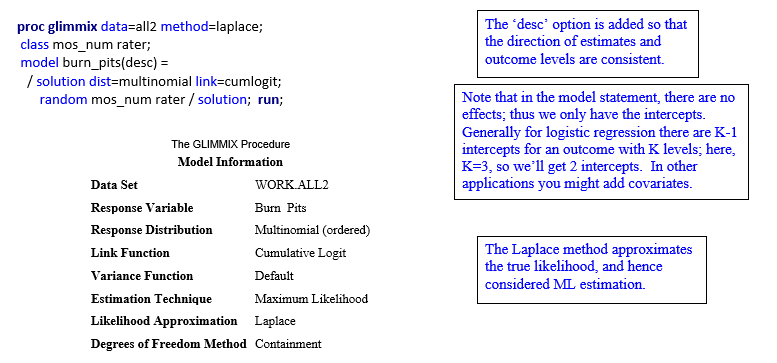
\includegraphics[width=0.8\linewidth]{figs_L17/f1} \end{center}
\end{frame}

\begin{frame}{}
\protect\hypertarget{section-2}{}
\begin{center}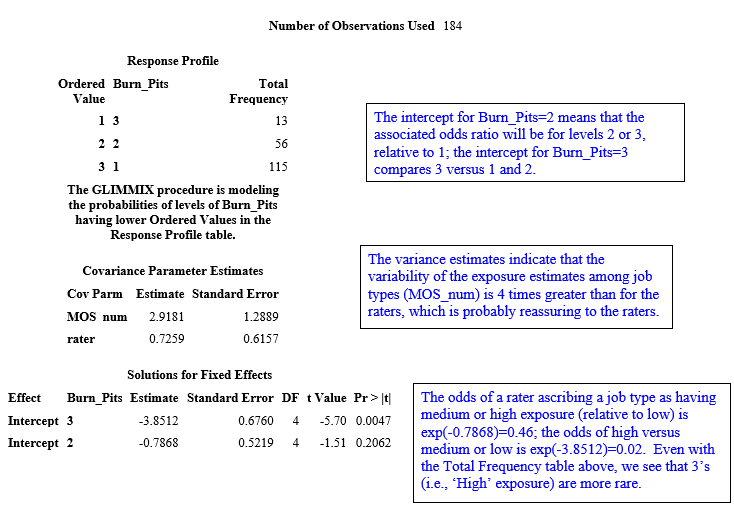
\includegraphics[width=0.8\linewidth]{figs_L17/f2} \end{center}
\end{frame}

\begin{frame}{}
\protect\hypertarget{section-3}{}
\begin{center}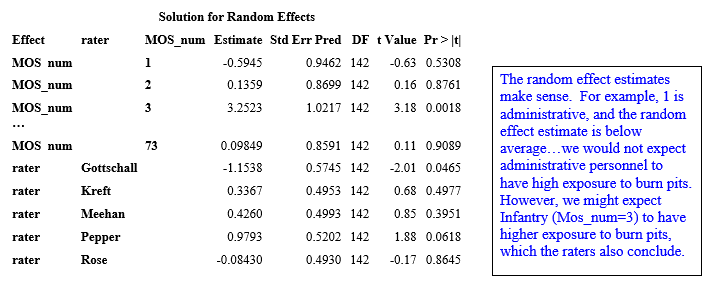
\includegraphics[width=0.6\linewidth]{figs_L17/f3} \end{center}

We see that Pepper scores job types higher, on average, with respect to
Burn pit exposure, compared with the average rater; similarly,
Gottschall scores lower. These both occur with marginal significance.
\end{frame}

\begin{frame}{}
\protect\hypertarget{section-4}{}
From our ordinal logistic regression model, we note that
\(P(Y_{ij} \geq k\ |\ b_i,\ b_j)=\frac 1 {1+e^{-\lambda_{ijk}}}\) and
\(P(Y_{ij} \geq k|b_i=0,\ b_j=0)=\frac 1 {1+e^{-\alpha_k}}\). From the
latter, we can estimate that for an average rater and MOS\_num, the
probability of `high' classification is
\(\frac 1 {1+e^{3.8512}} = 0.02\).

Job and rater-specific probability estimates can be obtained by using
the first formula. We can also compute for specific MOS\_num or raters,
holding the other at its mean, since random effects are crossed. For
example, for an average MOS\_num the probability of a high
classification for Gottschall is
\(\frac 1 {1+e^{-(-3.8512-1.15)}} = 0.7\%\), while for Pepper it is
\(\frac 1 {1+e^{-(-3.85+0.98)}} = 5.4\%\).

We can get probabilities for any given level by computing the cumulative
probabilities, and then taking differences {[}e.g.,
\(P(Y=2)=P(Y \geq 2) - P(Y \geq 3).\){]}
\end{frame}

\begin{frame}{Comparing the descriptive and modeled approaches}
\protect\hypertarget{comparing-the-descriptive-and-modeled-approaches}{}
Going back to the probabilities and odds we determined for the
descriptive approach, why do they differ from the modeled approach?
Descriptive: \(P(M\ or\ H)=37.5\%\) \(Odds(M\ or\ H)=0.6\)\\
\(P(H) = 7.1\%\) \(Odds(H)=0.076\)\\
Modeled: \(P(M\ or\ H)=31.3\%\) \(Odds(M\ or\ H)=0.46\) \(P(H) = 2\%\)
\(Odds(H)=0.02\)

Why the difference? It appears that taking the correlation into account
affects results; if the random effects are removed, here is what we get
from the model (same as descriptive, above): Modeled:
\(P(M\ or\ H)=37.5\%\) \(Odds(M\ or\ H)=0.6\)\\
\(P(H) = 7.1\%\) \(Odds(H)=0.076\)
\end{frame}

\begin{frame}{Using the mixed-effects ordinal logistic regression for
longitudinal data}
\protect\hypertarget{using-the-mixed-effects-ordinal-logistic-regression-for-longitudinal-data}{}
We can generalize the formula for the mixed-effects ordinal logistic
regression model so that it can be used for clustered / longitudinal
data and include covariates. One such model that is useful for repeated
measures within subjects (or subjects within clusters) is
\(\lambda_{ijk}=log\Big[\frac {P(Y_{ij}\leq k\ |\ \pmb b_i)} {1-P(Y_{ij}\leq k|\pmb b_i)} \Big] = \alpha_k + \pmb x_{ij}^r \pmb \beta+ \pmb z_{ij}^r \pmb b_i\)

where \(i\) denotes subject, with measure \(j\) (or subject \(j\) in
cluster \(i\)). Here, we have hierarchical data and so the random
effects (as is usually done) are defined for the level 2 data
(subjects).
\end{frame}

\begin{frame}{}
\protect\hypertarget{section-5}{}
The previous model can be used for longitudinal ordinal logistic
regression, although we only account for repeated measures via random
effects. (Using pseudo-likelihood methods, you could consider models
that account for random effects or serial correlation, or both.)

Now we have what is called a proportional odds model (see McCullagh,
1980) that results from the fact that the relationship between the
cumulative logit and the predictors does not depend on k.

For example, say that the previous case study also had measurements over
time (\(x\)=time). If we added this as a predictor, then the cumulative
logits (and hence probabilities) would not change over time.
\end{frame}

\begin{frame}{}
\protect\hypertarget{section-6}{}
We can generalize the model slightly so that for certain predictors, we
do not require the proportional odds assumption.

For example, Hedeker and Mermelstein (1998, 200) suggest the model
\(\lambda_{ijk}=log \Big[\frac {P(Y_{ij} \leq k\ |\ \pmb b_i)} {1-P(Y_{ij}\leq k\ |\ \pmb b_i)} \Big]= \alpha_k + \pmb x_{ij}^r \pmb \beta + \pmb s_{ij}^r \pmb \gamma_k + \pmb z_{ij}^r \pmb b_i\),
where the additional term involving \(\gamma_k\) allows the effects for
the associated covariates to vary across the cumulative logits.

For more detail, see the above references or Hedeker and Gibbons (2006).
Hedeker does warn about use of this partial proportional odds model,
with respect to inference for certain values of the covariates. For more
detail, see Hedeker and Gibbons (2006).
\end{frame}

\hypertarget{summary}{%
\section{Summary}\label{summary}}

\begin{frame}{Summary}
\protect\hypertarget{summary-1}{}
\end{frame}

\end{document}
